% Gallery figure source
% Summary: Horizontal gene transfer and homologous recombination are distinct. HGT can add DNA without replacing a homologous region, while homologous recombination after transfer can replace a recipient tract with donor-derived DNA. Green marks DNA not adopted by the recipient.
\documentclass[tikz,border=6pt]{standalone}
% Shared color palette
\usepackage[T1]{fontenc}
\usepackage[utf8]{inputenc}
\usepackage{lmodern}
\usepackage{microtype}
\usepackage{amsmath,amssymb,mathtools}
\usepackage{xcolor}
\usepackage{tikz}
\usetikzlibrary{arrows.meta,positioning,calc,fit,backgrounds,decorations.pathreplacing,shapes.geometric,shadows.blur}

\definecolor{mainblue}{RGB}{42,85,132}
\definecolor{deepgreen}{RGB}{30,105,70}
\definecolor{burntorange}{RGB}{190,90,25}
\definecolor{softgray}{RGB}{245,246,248}
\definecolor{darkgray}{RGB}{70,70,70}
\definecolor{violet}{RGB}{110,70,150}

\newcommand{\given}{\,|\,}
\newcommand{\Ne}{N_{e}}
\newcommand{\ARG}{\mathrm{ARG}}
\newcommand{\MRCA}{\mathrm{MRCA}}
\newcommand{\GMRCA}{\mathrm{GMRCA}}

% Shared TikZ styles
\tikzset{
  tip/.style={circle,fill=black,inner sep=1.6pt},
  nodept/.style={circle,fill=black,inner sep=1.4pt},
  sampled/.style={rectangle,fill=black,inner sep=2.2pt},
  branch/.style={line width=0.8pt},
  retic/.style={circle,draw=burntorange,fill=burntorange!25,line width=0.8pt,inner sep=2.0pt},
  event/.style={circle,draw=mainblue,fill=mainblue!15,line width=0.8pt,inner sep=1.8pt},
  arr/.style={-{Latex[length=2.0mm]},line width=0.8pt},
  faint/.style={line width=0.7pt,draw=gray!55},
  parentedge/.style={-{Latex[length=2.0mm]},line width=0.9pt,draw=burntorange},
  treeedge/.style={-{Latex[length=2.0mm]},line width=0.9pt,draw=black},
  segment/.style={line width=4pt,line cap=round},
  dashedretic/.style={-{Latex[length=2.0mm]},line width=0.9pt,draw=burntorange,dashed}
}


\begin{document}
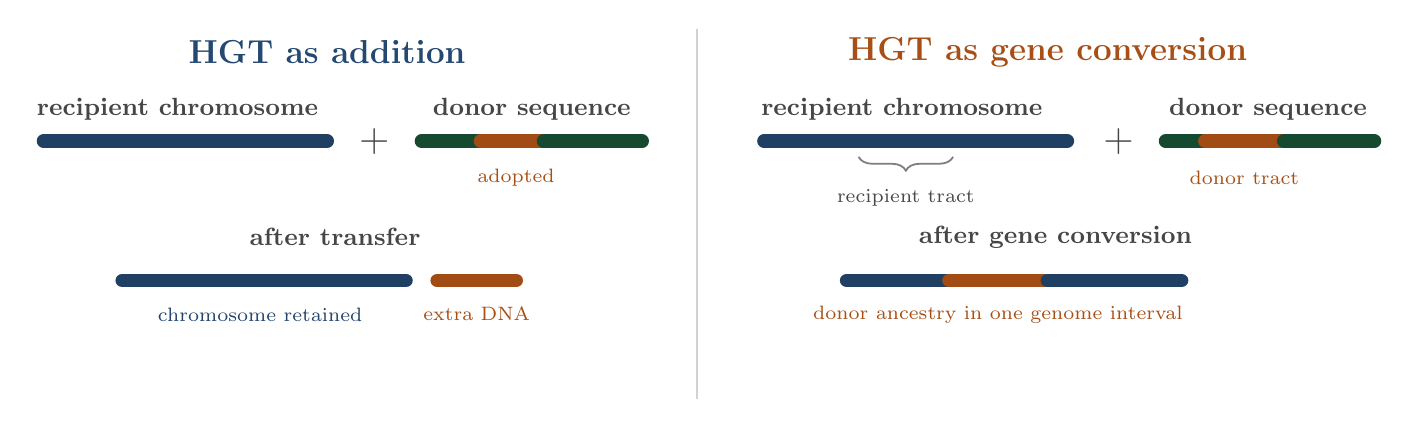
\begin{tikzpicture}[
  scale=1.0,
  chrom/.style={line width=5.0pt,line cap=round},
  adopted/.style={draw=burntorange!85!black},
  recipient/.style={draw=mainblue!75!black},
  unused/.style={draw=deepgreen!70!black},
  paneltitle/.style={font=\bfseries\large},
  smallnote/.style={font=\scriptsize,align=center,text=darkgray},
  midlabel/.style={font=\small\bfseries,text=darkgray},
  resultlabel/.style={font=\small,align=center,text width=5.6cm,text=darkgray},
  brace/.style={
    decorate,
    decoration={brace,amplitude=5pt,mirror},
    line width=.65pt,
    draw=darkgray!70
  },
  plus/.style={font=\Large\bfseries,text=darkgray}
]

\begin{scope}
  \node[paneltitle,text=mainblue!85!black] at (3.95,3.35)
    {HGT as addition};

  \node[midlabel] at (2.05,2.62) {recipient chromosome};
  \draw[chrom,recipient] (0.35,2.22)--(3.95,2.22);

  \node[plus] at (4.55,2.22) {$+$};

  \node[midlabel] at (6.55,2.62) {donor sequence};
  \draw[chrom,unused]  (5.15,2.22)--(5.90,2.22);
  \draw[chrom,adopted] (5.90,2.22)--(6.70,2.22);
  \draw[chrom,unused]  (6.70,2.22)--(7.95,2.22);

  \node[smallnote,text=burntorange!88!black] at (6.35,1.76)
    {adopted};

  \node[midlabel] at (4.05,1.00) {after transfer};

  \draw[chrom,recipient] (1.35,0.45)--(4.95,0.45);
  \draw[chrom,adopted]  (5.35,0.45)--(6.35,0.45);

  \node[smallnote,text=mainblue!80!black] at (3.10,0.02)
    {chromosome retained};
  \node[smallnote,text=burntorange!88!black] at (5.85,0.02)
    {extra DNA};
\end{scope}

\draw[gray!35,line width=.6pt] (8.65,-1.05)--(8.65,3.65);

\begin{scope}[xshift=9.15cm]
  \node[paneltitle,text=burntorange!88!black] at (3.95,3.35)
    {HGT as gene conversion};

  \node[midlabel] at (2.10,2.62) {recipient chromosome};
  \draw[chrom,recipient] (0.35,2.22)--(4.20,2.22);

  \draw[brace] (1.55,2.02)--(2.75,2.02)
    node[midway,below=8pt,font=\scriptsize,text=darkgray]
    {recipient tract};

  \node[plus] at (4.85,2.22) {$+$};

  \node[midlabel] at (6.75,2.62) {donor sequence};
  \draw[chrom,unused]  (5.45,2.22)--(5.95,2.22);
  \draw[chrom,adopted] (5.95,2.22)--(6.95,2.22);
  \draw[chrom,unused]  (6.95,2.22)--(8.10,2.22);

  \node[smallnote,text=burntorange!88!black] at (6.45,1.76)
    {donor tract};

  \node[midlabel] at (4.05,1.00) {after gene conversion};

  \draw[chrom,recipient] (1.40,0.45)--(2.70,0.45);
  \draw[chrom,adopted]  (2.70,0.45)--(3.95,0.45);
  \draw[chrom,recipient] (3.95,0.45)--(5.65,0.45);

  \node[smallnote,text=burntorange!88!black] at (3.32,0.02)
    {donor ancestry in one genome interval};
\end{scope}

\end{tikzpicture}
\end{document}
